\chapter{Machine Learning}
\label{chap:machine_learning}


\newpage

\section{Fundamentals}
The field of Machine Learning is concerned with algorithms which are able to `learn' from experience, this may be contrasted with algorithms which achieve some task with a set of static instructions. The ability to learn allows these algorithms to solve problems which may be too complex for a collection of explicity defined instructions. 
This chapter will give an overview of machine learning as pertinent to the field of high-energy physics. We begin with the fundamentals of machine learning, then move on to ensembling and decision trees, and finally neural networks and deep learning.  


\subsection{The Learning Process}

\subsubsection{Problem Formulation}
The data in a machine learning problem are often formulated in terms of a vector space $X = \mathds{R}^{n}$, where each dimension is an observable quantity referred to as a `feature' and a particular datum corresponds to a single feature vector $\vec{x} \in X$. A dataset is represented as a set of feature vectors $\vec{x}_{i}$.
A machine learning algorithm can then be considered to consist of a model $f$, 
\begin{equation}
    f:(X,\vec{w})\rightarrow{Y}
\end{equation}
which is a function that maps from a feature vector $\vec{x}$ to an outcome $Y$ given a vector of parameters $\vec{w}$; a loss function $L$
\begin{equation}
    L:(f,\vec{x}_{i})\rightarrow{\mathds{R}}
\end{equation}
which measures performance given the model, a set of feature vectors and sometimes the desired outcome; 
and finally, an optimisation which alters the parameters of the model given the loss to drive the learning process.


Learning is said to be occur when the model's performance at some class of tasks $T$ as measured by some performance measure $P$ improves given experience $E$. 
There are many classes of task which depend on the dataset and the desired outcome, but the two main classes of interest are classification and regression:
\begin{itemize}[leftmargin=.5in,noitemsep]
    \item Classification tasks aim to predict a class given a feature vector, $f:\mathds{R}^{n}\rightarrow{}\{1,\dots,k\}$.
This is often an integer class label but can be a probability distribution over classes. An example of a classification problem from physics would be signal-background event discrimination where we attempt to classify events into background-like or signal-like classes.
    \item Regression tasks aim to predict a continuous value given the input features, $f:\mathds{R}^{n}\rightarrow\mathds{R}$. An example of a regression task in physics would be detector calibration where we attempt to predict the true value from the measured. 
\end{itemize}
In addition to these main classes of task there are others such as structured prediction that attempts to predict more complicated structures such as trees and lists, and many others. 


The experience that the model recieves depends on the data that the model is exposed to during optimisation, and can be split into two broad categories:
\begin{itemize}[leftmargin=.5in,noitemsep]
    \item Supervised machine learning algorithms experience target values $y$ as well as the input features $x$. They will experience multiple examples of feature vectors and attempt to reconstruct the correct value, with the loss calculated given the target. An example would be a classifier which is simulated data where we know the true signal-background class label. 
    \item Unsupervised algorithms do not have access to target values and will attempt to infer information about the structure of the data such as clusters.
\end{itemize}



\subsubsection{Training and Evaluation}

The learning process is also referred to as `training' and has a different objective to a typical optimisation problem: rather than just finding the parameters which give the optimal loss over the training dataset, we require the model to find useful behaviours that generalise to new data. 
To estimate the generalisation power of a model, we evaluate performance over another unseen dataset, the test set, which should be chosen such that it is representative of the distribution of the whole dataset.


During training most machine learning algorithms will use some form of gradient-based optimisation where one descends the gradient of $L$ with respect to $\vec{w}$ to find the minimum of $L$,
\begin{equation}
    \nabla_{\vec{w}}L = 0.
\end{equation}
The most conceptually simple approach is to evaluate this expression over the entire training set, however this is often impractical for large datasets which have a large population or high dimensionality. 

An alternative is to use stochastic gradient descent (SGD). With SGD we descend the gradient in steps where each step is performed by evaluating the gradient with small batches of training data (minibatches). 
The parameters are then updated as
\begin{equation}
    \vec{w} \rightarrow \vec{w} - \eta\nabla_{\vec{w}}L
\end{equation}
where $\eta$ is the learning rate, a parameter that controls the size of the steps at each parameter update. As we repeat this step the model parameters should ideally converge to a global optimum, but there are often local optima that the training can get settle into. To avoid these we must tune our model carefully and apply our prior knowledge. 


\subsubsection{Example: linear regressor}
Now we have the ingredients of a machine learning algorithm, consider the simple example of a linear regressor. 

The dataset will consist of n-many points of single features, and the value to predict. The are distributed as a linear function with $\vec{w} = (-2,2)$ and a random noise component drawn from a Gaussian distribution

The task of linear regression is to predict the value $y$ given a collection of features. In this formulation we will consider a single feature $x$, and the algorithm will have access to the $y$ during training making this a supervised learning problem. 

The formula of the model is
\begin{equation}
    \hat{y} = w_{1} + w_{2}x
\end{equation},
linear refers to the model parameters not the features these can be any power of $x$ too, 
the loss will be the mean squared error,
\begin{equation}
    L = \frac{1}{n}\sum_{i=1}^{n}(\hat{y}_{i}-y_{i})^{2}
\end{equation}
The experience will be optimisation of MSE with SGD over the training set and then the performance measure will be loss evaluated on the test set. 
A single SGD step will be 
\begin{equation}
    \begin{pmatrix}
        w_{1} \\
        w_{2}
    \end{pmatrix} \rightarrow
    \begin{pmatrix}
        w_{1} \\
        w_{2}
    \end{pmatrix} - \eta
    \frac{1}{m}\sum_{i=0}^{m}
    \begin{pmatrix}
        2(w_{1}+w_{2}x_{i} - y_{i})\\
        2x_{i}(w_{1}+w_{2}x_{i} - y_{i})
    \end{pmatrix}
\end{equation}
where $m$ is the minibatch size.

The training is performed for $500$ minibatches with a learning rate of $0.0001$ and parameters initialised to $1$. The training process and final outcome of this algorithm are shown in Figure \ref{fig:machine_learning:lin_example}.

\begin{figure}[h!]
    \begin{center}
        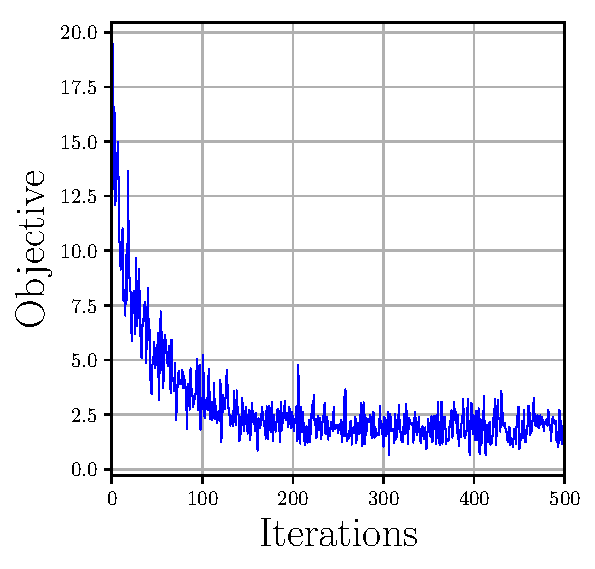
\includegraphics[width=0.32\textwidth]{figures/machine_learning/loss_history.pdf}
        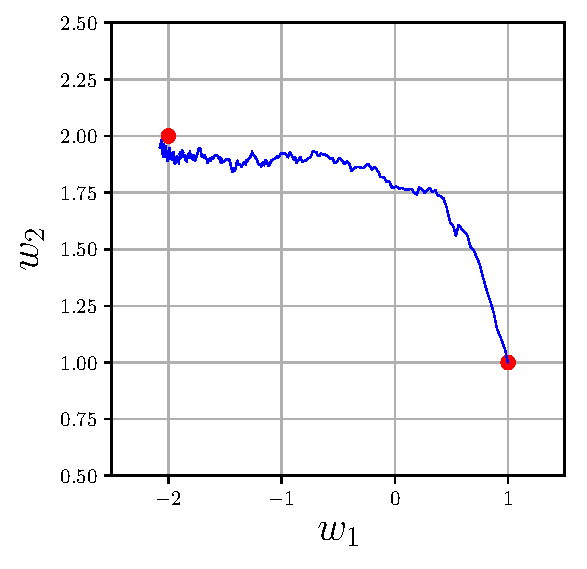
\includegraphics[width=0.32\textwidth]{figures/machine_learning/w1_w2_history.pdf}
        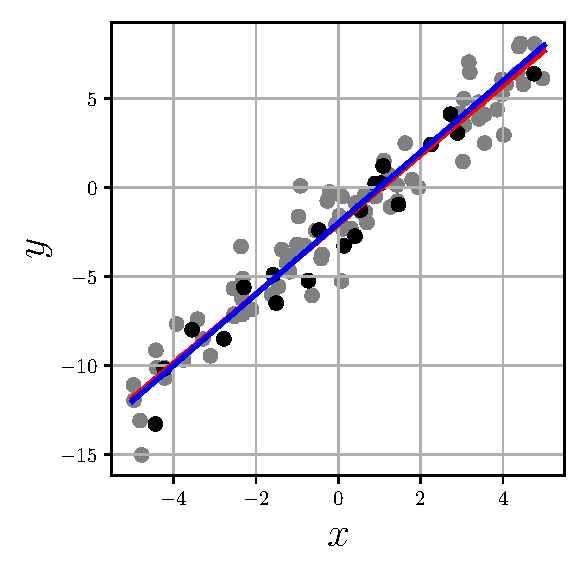
\includegraphics[width=0.32\textwidth]{figures/machine_learning/data_and_results.pdf}
    \end{center}
    \caption{Training a linear regressor. Loss history over training (left), the trajectory of the model parameters in parameter space during training (centre), and the final result with the result in read and the true value in blue, an example minibatch is shown by the black points (right).}
        \label{fig:machine_learning:lin_example}
\end{figure}








\subsection{Model Capacity and Generalisation}
The example of a linear regressor can be expanded to use higher-order polynomials,
\begin{equation}
    \hat{y} = \sum_{i=0}^{N}w_{i}x^{i}.
\end{equation}
When we do this we have increased the space of functions (the hypothesis space) which the model can draw upon to describe the observed datapoints, this is called model capacity.
When the capacity of a model is inappropriately large or small for the dataset it can experience problems with generalisation.
(talk about training error and test error here)
If the capacity is too small this leads to `underfitting' where the model does not have enough descriptive power to fit the data, if there is too much capacity the model will find a function fit to the training set arbitrarily well but will fail to generalise, this is `overfitting. Examples of how inapropriate capacity can lead to a failure to generalise are shown in Figure \ref{fig:machine_learning:overfitting}.
\begin{figure}[h!]
        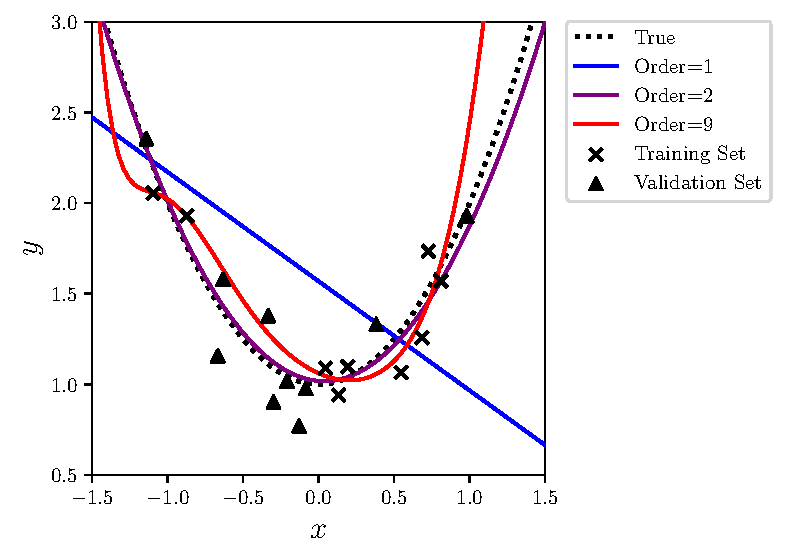
\includegraphics[width=0.65\textwidth]{figures/machine_learning/capacity.pdf}
    \caption{Linear regressors with different order polynomials fitted to the same data. }
        \label{fig:machine_learning:overfitting}
\end{figure}


To control capacity one can reduce or extend the hypothesis space by adding or removing functions that the model can use. In the example of the linear regressor this correspond to changing the order of the polynomial. 

An alternative and more general approach to controling model capacity is to penalise parts of the hypothesis space rather than remove them. This way, if we have two functions which perform equally well, we can express some sort of preference for which one to choose by adding a term to the loss. This penalty term is called a `regularizer' term and has the form
\begin{equation}
    \lambda\Omega(\vec{w}),
\end{equation}
where $\lambda$ is a value which scales the strength of the regularizer's effect. Removing functions from the hypothesis space can be considered to be an infinite penalisation. These terms are examples of regularisation which is a broad class of techniques with the purpose of improving the generalisation error of a learning algorithm. 


Two common forms of regularisation are penalty terms based on the squared $L^{2}$ and $L^{1}$ norms of the model's weight vector
\begin{equation}
    \begin{split}
        \lambda||\vec{w}||^{2}_{2} =& \lambda\sum_{i=0}^{n}w_{i}^{2} \\
        \lambda||\vec{w}||_{1} =& \lambda\sum_{i=0}^{n}|w_{i}|. \\
    \end{split}
\end{equation}
These two regularizers have a different effect on the model parameters: $L^{2}$ regularization expresses a preference for using each parameter a small amount, $L^{1}$ regularization will prefer sparsity where a few parameters are large, and the rest close to zero. 
A comparison of a range of values for both regularizers is shown in Figure \ref{fig:machine_learning:reg_example}. Here we train a linear regressor on a quadratic function
\begin{figure}[h!]
    \begin{center}
        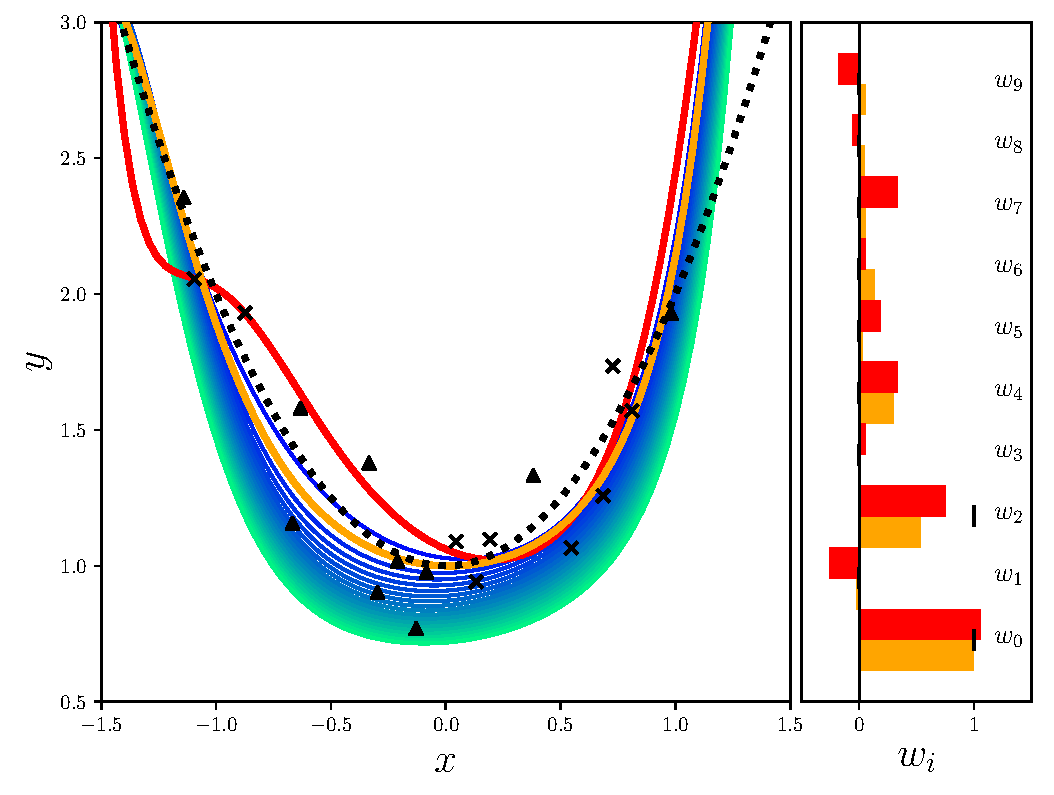
\includegraphics[width=0.49\textwidth]{figures/machine_learning/L2_reg_plot.pdf}
        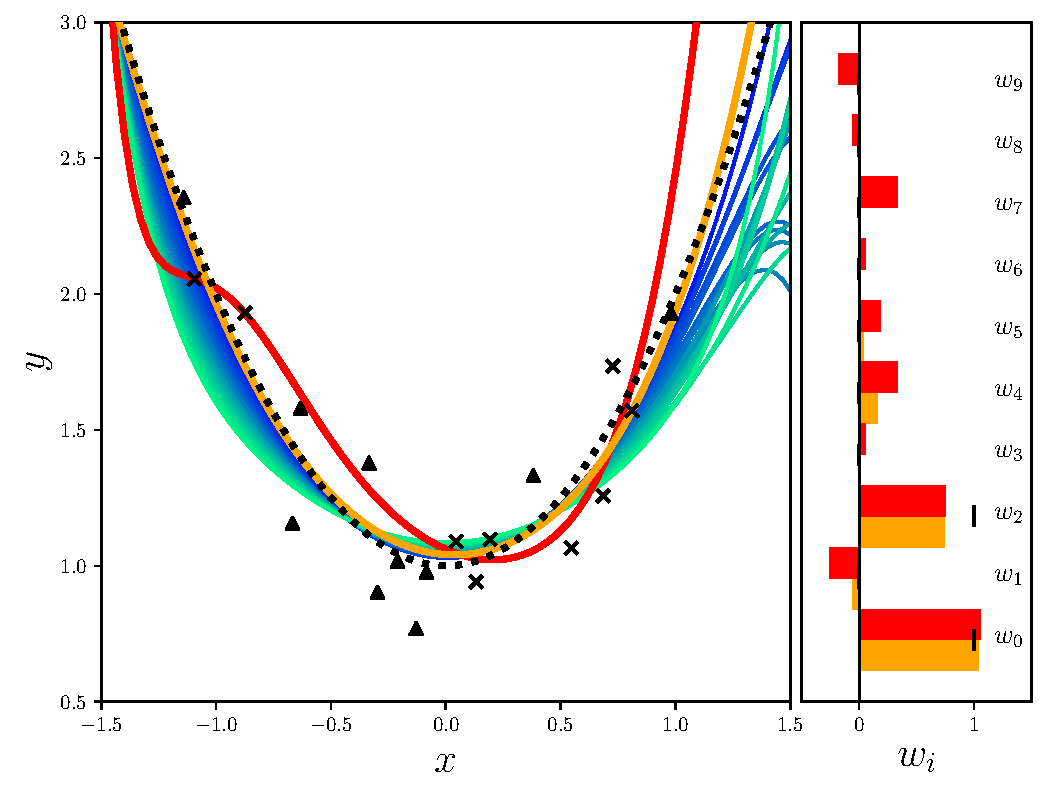
\includegraphics[width=0.49\textwidth]{figures/machine_learning/L1_reg_plot.pdf}
    \end{center}
    \caption{Fits for different regularisation strengths with $L^{2}$ (left) and $L^{1}$ (right) regularisation data drawn from a uniformly sample of $y=1+x^{2}$ plus noise. The red curve is the unregularised fit, the orange curve is the result with the lowest loss with respect to the validation set (triangles). The bar charts show the parameter values of the overfitted result and optimal regularised result.} 
        \label{fig:machine_learning:reg_example}
\end{figure}
One notes the different effect adjusting the strength of the regularizer has for both types: $L^{2}$ attempts to use all of the features a small amount, and $L^{1}$ picks out specific parameters to make large with the others being very close to zero. 

When we are designing a machine learning algorithm to solve a problem, regularization and the tuning other hyperparameters are of crucial importance alongside model selection. 


\subsection{Algorithm Design and Optimisation}

% No free lunch theorem
The No Free Lunch theorem of machine learning states that, averaged over all possible data-generating distributions, every classification algorithm has the same error rate when classifying previously unobserved points.
This result essentially means that no machine learning algorithm is universally superior, but it does not mean that they are all equally-powerful for a particular task. 
The theorem only holds averaged over all distributions, and some algorithms will indeed perform better given specific focus: we must make assumptions given prior knowledge and build our algorithms accordingly.
This will inform how we choose the model, how we measure performance, and how we optimise the hyperparameters. 


% Curse of dimensionality
A particularly important phenomenon is the `curse of dimensionality' where machine learning algorithms can under-perform given a dataset with a large number of features (high-dimensionality).
For such a dataset the number of possible configurations of the features are far larger than the size of the training set. 
This can also be formulated in terms of coverage of a hypervolume (Figure \ref{fig:machine_learning:curse_of_dimensionality}): if one considers a unit cube of dimension $D$, the portion of the sides required to cover a given volume increases rapidly with $D$.
This issue is a primary motivator for the development of deep learning, and is also something that needs to be considered during hyperparameter optimisation. 
\begin{figure}[h!]
    \begin{center}
        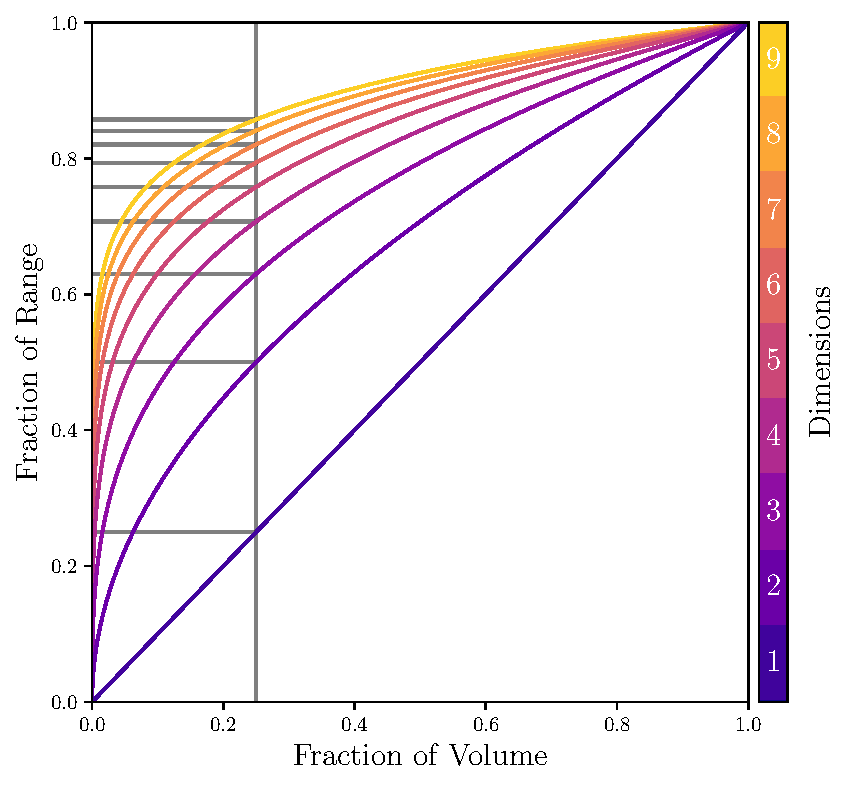
\includegraphics[width=0.49\textwidth]{figures/machine_learning/curse_of_dimensionality.pdf}
    \end{center}
    \caption{Range of the side length to cover a fraction of the volume of a unit cube in up to nine dimensions. The grey lines show the fraction required to cover 25\% of the volume.}
        \label{fig:machine_learning:curse_of_dimensionality}
\end{figure}


% What's to be designed? Model, objective, task, experience and constraints
Choice of model, and input features, will depend on a number of practical constraints such as time and computational resources, but also constraints that avoid biases particular to physics analyses. 
In training a classfier to separate Higgs boson signals on simulation we do not want the algorithm to reconstruct the mass and bias itself to the simulation value. This can happen if the algorithm is given this value explicitly or if it is capable to reconstructing it from the other features.  
Furthermore one must use assumptions from prior knowledge of dataset size, dimensionality and other properties such as linear separability and class balance to choose the model. One can then evaluate candidate algorithms using apropriate performance measures. 


% What's it designed with respect to? Performance measures
Performance measures depend on the task.
Accuracy is not a good measure (improper performance measure), ROC is good for overall but we might be interested in maximising purity, precision/recall and average precision is handy, loss is fine. 
All on the validation set. 

% Hyperparameters
Hyperparameters can be selected with a variety of optimisation approaches, but because the underlying function which maps from hyperparameters to performance values is unknown we cannot use gradient-based methods. Here we use derivative-free optimisation methods, two of which will be presented here and used later in this thesis: grid search and Bayesian optimisation.

% Optimisation with grid search
Grid search is a simple method which simply samples a set of evenly-spaced values over a given region of the hyperparameter space. 
This method can be used when there are fewer hyperparameters to optimise and the time cost of sampling each point is not too great. 
As the number of hyperparameters goes up, dimensionality increases and the sampling becomes extremely sparse as each point represents a smaller portion of the space.

% Optimisation with Bayesian Optimisation
Bayesian optimisation is part of a class of optimisation algorithms that use previous observations of the performance to determine the next point to sample. 
The method consists of two main steps (for detail see Appendix A):
\begin{enumerate}[leftmargin=.5in,noitemsep]
    \item using evaluated points in the hyperparameter space calculate a posterior expectation of the performance as a function of the hyperparameters
    \item evaluate the performance at a new point which maximises an 'acquisition function', a function which scores how optimal a point in the hyperparameter space is to evaluate. 
\end{enumerate}
Bayesian optimisation makes efficient use of sampling and is more apropriate when evaluating a single point in the hyperparameter space is expensive. 

These two methods can be combined where an initial grid search is performed, and the set of evaluated points are used in the first iteration of the Bayesian optimisation. 
This step is called a `warm start'. 



\subsection{Ensembles}

%Ensembles: what and why?
Ensembles are another approach to constructing a strong classifier. This uses many weaker classifiers combined together to achieve superior performance. 

%Decision Trees
Decision trees repeatedly partition the feature space

%Boosting
Gradient boosting works as follows...

\section{Deep Learning}

\subsection{Neural Networks}

\subsection{Training and Regularisation}

\subsection{The problems of depth}

\subsection{Convolutional Neural Networks}
